\chapter{Das Framework TensorFlow}

\gls{TF} ist eine plattformunabhängige Bibliothek für \gls{ML}, die für große und variable Architekturen entwickelt~\cite{tensorflow2015-whitepaper} und Ende 2015 veröffentlicht wurde~\cite{tf-opensource}. Um die einzelnen Verarbeitungsschritte der Daten darzustellen, werden von \gls{TF} sogenannte Datenfluss Graphen verwendet. Diese bieten auch die Möglichkeit für alle Operationen festzulegen, von welcher Hardware sie berechnet werden sollen. \gls{TF} unterstützt dabei CPUs, GPGPUs\footnote{general-purpose graphics processing units} und eigens für \gls{ML} entwickelte Hardware.
%http://www.cs.virginia.edu/~gurumurthi/papers/DATE14.pdf
Besonders umfangreich unterstützt das Framework Arbeiten im Bereich der (tiefen) \gls{NN}. Schnittstellen zu den Hochsprachen Python und C++ sollen den Einstieg erleichtern und sicherstellen, dass die verfügbare Hardware immer bestmöglich genutzt werden kann. Mit dem sogenannte Tensorboard bringt \gls{TF} außerdem eine Weboberfläche mit, die ohne großen Aufwand für den Entwickler viele relevante Informationen ausgibt und teilweise auch grafisch aufbereitet~\cite{tensorflow2016-whitepaper}.

\section{Eine Einführung zu TensorFlow}

%evtl. Vergleich mit anderen Frameworks (CAFFE, Torch, ...)

\section{Die Entwicklung von Tensorflow}
Bereits 2011 begann das Google Brain Projekt damit, den Nutzen von sehr großen tiefen \gls{NN} zu erforschen. Einen Teil davon bildete der Aufbau von "`DistBelief"', ein System, das Training und Vorhersage im Bereich des \gls{ML} verteilt und skalierbar ermöglichte. Neben einigen Forschungsprojekten wurde DistBelief auch bereits produktive in einigen Google Produkten, wie Google Search, Google Tanslate oder Youtube eingesetzt~\cite{tensorflow2016-whitepaper}. 2012 wurde von Google Mitarbeitern ein Paper veröffentlicht, das über die Nutzung von zentausenden CPU-Kernen  durch DistBelief berichtete, wodurch auch sehr große Modelle in absehbarer Zeit trainiert werden konnten~\cite{NIPS2012}. Auf Basis der Erfahrungen beim Einsatz von DistBelief arbeitete Google dann am System der zweiten Generation für groß-skalierende \gls{ML} Modelle und veröffentlichte im November 2015 \gls{TF}~\cite{tf-opensource}. \gls{TF} ist seit dem auf github unter der Apache License 2.0 verfügbar~\cite{tf-git}.  Mit der Veröffentlichung von Version 1.0 im Februar 2017 wurde schließlich eine verlässliche API eingeführt, die auch in Zukunft sicher stellen soll, dass der geschriebene Code mit neuen Versionen von \gls{TF} kompatibel ist~\cite{tf1}. Des weiteren wurde die Leistung weiter verbessert und die Einführung eines neuen Moduls ermöglicht seither die Nutzung von \gls{TF} mit Keras\footnote{Keras ist eine Deep Learning Library, die auf \gls{TF}, CNTK oder Theano aufsetzt.}.

\section{Angesprochene Zielgruppe}
Im Gegensatz zu DistBelief, welches viele Forschungsgebiete zu unflexibel war, ist \gls{TF} sowohl für die Forschung als auch für den Produktiven Einsatz in großen Softwareprojekten geeignet. \autoref{fig:DBvsTF} wurde beim TensorFlow Dev Summit 2017~\cite{tf-sum17-keynote} gezeigt und veranschaulicht die Abdeckung der Zielgruppen beider Systeme.

\begin{figure}[htb!]
	\centering
	 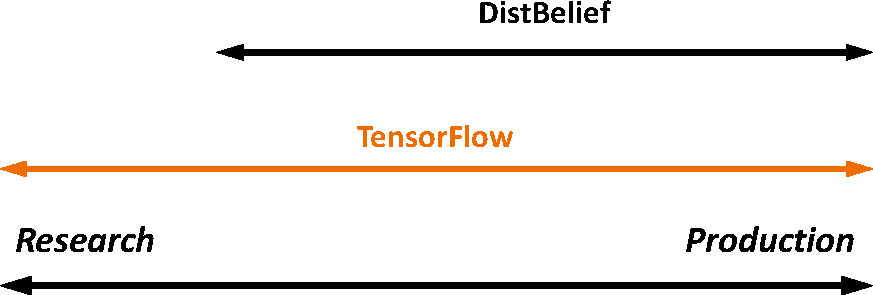
\includegraphics[width=.7\textwidth]{images/DistBeliefvsTensorFlow.pdf}\\
	\vspace{10pt} 
	\caption{Zielgruppenabdeckung von DistBelief und \gls{TF}~\cite{tf-sum17-keynote}}
	\label{fig:DBvsTF}
\end{figure}

\gls{TF} bietet zum einen genug Flexibilität für Forschungsprojekte, um mit neuen Modellen zu experimentieren, ist gleichzeitig aber hochperformant und robust, was beim Einsatz in Produktivsoftware wichtig ist. Modelle können somit also oft aus der Forschung direkt in Produktivumgebungen übernommen werden~\cite{tensorflow2016-whitepaper}.


\section{Hard- und Software Anforderungen}



\subsection{Hardware Anforderungen}
%-CPU
%-GPU (nvidia mit CUDa support)
%-TPU
%-FPGA
\subsection{Software Anforderungen}


\section{Softwarearchitektur von TensorFlow}